\section{Simple measures of responsiveness}
\label{sec:responsiveness}

\subsection{Thresholding $|U_{10}|^2$ responsiveness}
\label{sec:thresh-resp}

As shown in Figure~19~of~T20~\cite{ZannaPreprint} (see Figure~\ref{fig:yin-responsiveness}),
they define a measure for `efficiency' (I prefer `responsiveness') based on Equation~\ref{eq:pugh},
by fitting a quadratic to daily wind speed vs.~surge height, with a threshold that they
vary between locations.
This threshold seems arbitrary,
so when I replicated this I chose that the $\Delta\eta_{\mathrm{hp}} \ge 0$,
as it approximately guarantees that the sea surface stress is acting into
the coast, and instead linearly fitted hourly $|U_{10}|$ against $\Delta\eta_{\mathrm{hp}}$,
with and without an intercept at the origin (Figure~\ref{fig:simple-responsiveness-results}).
The results for areas like Miami are similarly low, and for New Orleans are high,
so that Figure~\ref{fig:simple-responsiveness-results} seems to qualitatively reproduce the
results of Figure~\ref{fig:yin-responsiveness}. The lines were fitted on
2005's data due to it's higher Kurtosis (Figure~\ref{fig:ssh_stats_america}), and tested on
2004's data.\footnote{Based on the heuristic that
an ML algorithm performs better if trained on more interesting data.}
As can be seen in the bottom plot of Figure~\ref{fig:simple-responsiveness-results}
this generalises reasonably in some points (e.g. NO), but in areas where responsiveness was
low it generalises poorly.


\subsection{$\tau_u$, $\tau_v$ responsiveness}
\label{sec:tau-tau}
This method is quite crude, and I attempt to improve it by
using $\tau_u$ and $\tau_v$ with $\Delta\eta_{\mathrm{hp}}$.
After applying a number of linear regression algorithms ~\ref{fig:tau-tau-r-no},
I settle on \texttt{MLR} and \texttt{huber} as being the most reliable (see §~\ref{sec:lin-ml-models}).
I apply this along \texttt{eUS} in
Figure~\ref{fig:tau-tau-resp}, where the estimates produces by the
two different algorithms and trained on either year provide an estimate
for the confidence envelope.
Figure~\ref{fig:tau-tau-responsiveness}
creates a more robust metric for the responsiveness, by
taking the norm of the linear regression coefficients, and multiplying it
by the generalisation score, as I found that for \texttt{vc}
there are areas with v.~low scores and high regression coefficients which are spurious.

\begin{figure}
\centering
\includegraphics[width=1\linewidth]{../surge/plots/3d_plots/3d_plotnorlean.pdf}
 \caption{New Orleans \texttt{tyr} fit for 2005 (red) and 2004 (blue) using
 \texttt{huber}, \texttt{MLR}, \texttt{RANSAC} and \texttt{Theil-Sun}~\cite{scikit-learn}.
 \texttt{huber} and \texttt{MLR} are the most reliable, so are used further in later
 sections.}
 \label{fig:tau-tau-r-no}
\end{figure}


\begin{figure*}[htb!]
    \centering
    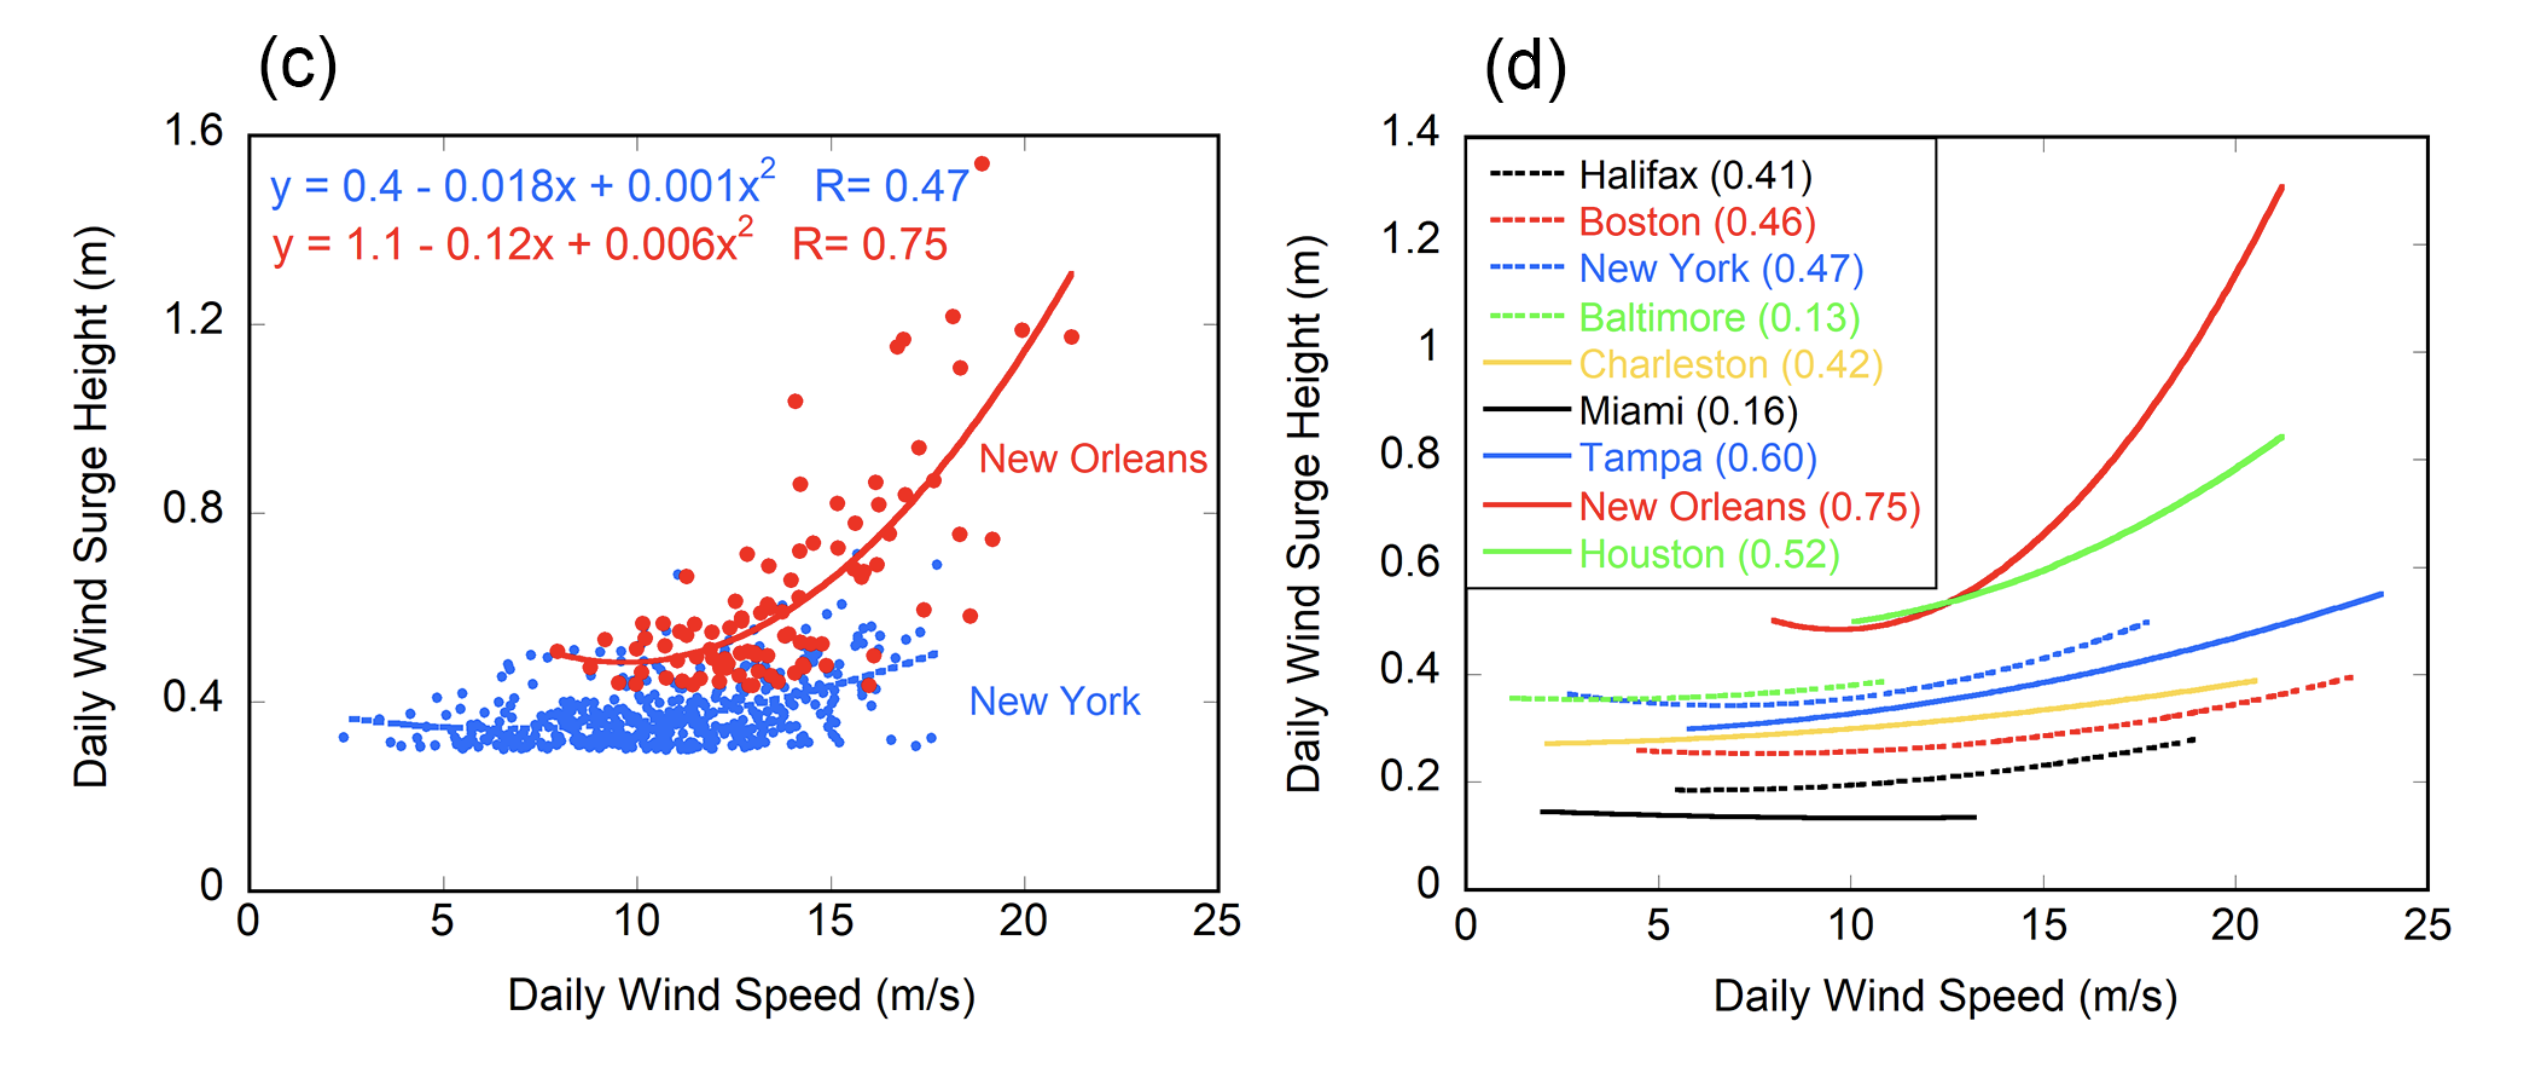
\includegraphics[width=0.8\linewidth]{images/example-images/yin-responsiveness.png}
    \vspace{-7pt}
    \caption{Figure 10c \& 10d in Yin et al.~2020~\cite{ZannaPreprint}. }
   \label{fig:yin-responsiveness}

   \includegraphics[width=0.8\linewidth]{../surge/plots/score-plot/score_plot.pdf}
   \vspace{-7pt}
   \caption{Linear Regression of $ \Delta \eta$ against $|U|^2$ for $ \Delta\eta>0$.
   Only generalises for the most vulnerable points. Most variance not modelled.}
  \label{fig:simple-responsiveness-results}
\end{figure*}




\begin{figure*}
\centering
 \hspace{-40pt} \includegraphics[width=0.6\linewidth]{../surge/plots/rmlr.pdf}
  \vspace{-15pt}
 \caption{A four panel plot to show the estimation of responsiveness
          of $\Delta\eta_{\mathrm{hp}}$ to $\tau_u$ and $\tau_v$, with the
          \texttt{MLR} and \texttt{Huber} algorithms. The y-units of A~\&~B are
           m Pa$^{-1}$.}
 \label{fig:tau-tau-resp}
 \hspace{-40pt} \includegraphics[width=0.3\linewidth]{../surge/plots/reg_angle.png}
  \vspace{-15pt}
 \caption{This shows that for the majority of the coastline there is a close
 corresponce between the normal bearing of the coast and the regression line ($r_p=0.83\pm0.05$).
 \texttt{np.arctan2(c0, c1)}}
  \label{fig:tau-tau-angle}
  \hspace{-40pt} \includegraphics[width=0.5\linewidth]{../surge/plots/adj_reg_mag.pdf}
   \vspace{-15pt}
  \caption{A more robust measure of responsiveness magnitude.
  ($\bar{r^2}$)\texttt{*np.sqrt(np.square(c0) + np.square(c1))}. }
   \label{fig:tau-tau-responsiveness}
\end{figure*}


\label{sec:angle}

From either multiple linear regression line,
it is possible to work out the
direction that it points, using arctan2,
Figure~\ref{fig:tau-tau-angle}, and compare it to the bearing of the coast (see~§~\ref{sec:convexity}).
The difference between the regression direction and
the bearing might be explained through Ekman transport~\cite{hope2013hindcast}.


\label{sec:reg-metrics}

The magnitude of this regression line is correlated ($r_p=0.78\pm0.05$\footnote{ for `w.o an intercept' against the four MLR alternatives.}) between the two
(Figures~\ref{fig:simple-responsiveness-results},\&~\ref{fig:tau-tau-responsiveness}),
showing that there is some underlying property of the
coastline they illuminate.
 I use \texttt{lasso} and \texttt{ridge} regression
to learn the responsiveness for \texttt{vc} and \texttt{eUS} using the metrics of isobath
distance and coastal convexity (109 features) (§~\ref{sec:convexity}~\&~\ref{sec:bath-grad}).
These are dissimilar in Figures~\ref{fig:learnt-eus}~\&~\ref{fig:learnt-vc},
suggesting that the coastal metrics need more development before they can be
useful predictors.

\label{sec:generalisability}


\begin{figure}[htb!]
    \centering
    \includegraphics[width=0.7\linewidth]{../surge/plots/ridge_lasso.pdf}
    \vspace{-15pt}
   \caption{\texttt{eUS} regression learning.
    Although not for lasso, and the regression is not consistent.
            We also need another coast to see if this generalises.}
    \label{fig:learnt-eus}

    \centering
    \includegraphics[width=0.8\linewidth]{../surge/plots/vc_ridge_lasso.pdf}
    \caption{The same as above, but for the \texttt{vc} coastline.}
    \label{fig:learnt-vc}
\end{figure}




\FloatBarrier
